\documentclass[10pt, conference]{IEEEtran}
\IEEEoverridecommandlockouts
\usepackage{cite}
\usepackage{amsmath,amssymb,amsfonts}
\usepackage{algorithmic}
\usepackage{graphicx}
\usepackage{url}
\usepackage{textcomp}
\usepackage{xcolor}
\usepackage{tikz}
\usetikzlibrary{shapes, arrows, positioning, fit, backgrounds, calc}

% figures live in ./figs/
\graphicspath{{figs/}}

\begin{document}

\title{Altitude as a Fleet-Wide Coverage Control for UAV-Mounted 5G Serving Ground Robots: A Protocol-in-the-Loop Emulation Study in Open-Field Line-of-Sight Conditions}

\author{
\IEEEauthorblockN{Innocent N. Makhubela}
\IEEEauthorblockA{\textit{Dept. of Electrical Engineering} \\
\textit{University of Cape Town} \\
Cape Town, South Africa}
\and
\IEEEauthorblockN{Joyce Mwangama}
\IEEEauthorblockA{\textit{Dept. of Electrical Engineering} \\
\textit{University of Cape Town} \\
Cape Town, South Africa}
}

\maketitle

\begin{abstract}
UAV-mounted base stations (``nomadic nodes'') can restore on-demand 5G connectivity to ground robots in search-and-rescue (SAR) operations, but system-level evidence of how such air-to-ground (A2G) links behave under continuous three-dimensional mobility and realistic traffic is scarce, and most prior work is analytic or link-level. We present an emulation testbed that couples a physics simulator to a real 5G standalone protocol stack: robot and UAV motion continuously drive an analytic A2G path-loss model whose output is injected at runtime into an OpenAirInterface gNB and two UEs, over which genuine TCP, fixed-rate UDP video, and command-and-control (C2) traffic are measured in both directions. In a 7.5-hour open-field, line-of-sight (LoS) campaign of 2{,}222 samples spanning 4--140~m of range and 20--60~m of UAV altitude, the emulated channel tracks the analytic model to within 1.2~dB mean absolute error, is corroborated by UE-reported RSRP (correlation $-0.91$ to $-0.99$), and is cross-validated by the coincident throughput--distance curves of two independent runs at equal altitude. The central result, from a controlled altitude sweep, is that UAV \emph{altitude} is a powerful coverage control: climbing from 20~m to 60~m at mid-range recovers 12~dB of link margin, triples throughput, and moves the coverage cliff from ${\sim}65$~m to ${\sim}125$~m, extending the safe operating radius from 101~m to 163~m. Because raising altitude improves the elevation angle to every robot at once, it acts as a fleet-wide (common-mode) control, in contrast to horizontal repositioning, which trades link quality between distributed users; a controlled lateral-tracking comparison is left as complementary future work. We further quantify device-budget, traffic-class, and repositioning effects; give the complete geometry-to-signal formula chain; and document three silent-failure pitfalls of single-host RAN emulation with their remedies. All findings are scoped to open-field LoS; NLoS and cluttered terrain are ongoing work.
\end{abstract}

\begin{IEEEkeywords}
UAV communications, nomadic base station, 5G NR, air-to-ground channel, search and rescue, OpenAirInterface, network emulation.
\end{IEEEkeywords}

\section{Introduction}
Search-and-rescue (SAR) operations frequently occur where terrestrial network infrastructure is damaged, congested, or absent. A UAV carrying a base station---a \emph{nomadic node}---can restore connectivity on demand, serving ground robots that stream sensor data and live video to a command post while receiving navigation waypoints and safety-critical commands in return \cite{zeng2016wireless, zeng2019accessing, mozaffari2019tutorial}. The concept and its analytic A2G channel models are well established \cite{alhourani2014optimal, 3gpp36777}. What remains scarce is \emph{system-level} evidence: how does a complete 5G protocol stack---with its scheduler, link adaptation, hybrid ARQ, and radio-link-failure (RLF) machinery---behave when the three-dimensional geometry between an aerial cell and its mobile ground users changes continuously, and what does that imply operationally?

This paper answers that question empirically. Our contributions are: (1) a fully specified, mobility-coupled emulation architecture---the software stack, its inter-component communication, and the geometry-to-signal pipeline; (2) a detailed account of three silent-failure pitfalls encountered during construction, with diagnoses and remedies, offered as reusable lessons; and (3) an empirical characterization, over a 7.5-hour LoS campaign, that establishes UAV altitude as the primary coverage lever and quantifies device-budget, traffic-class, and repositioning effects, with an explicit interpretation of what each result means for a deployed system. The study is deliberately restricted to an obstacle-free field with persistent line of sight---the cleanest setting for isolating the altitude/range/link-budget relationships---with NLoS and cluttered environments as future work (Section~\ref{sec:conclusion}).

\section{Related Work}
Al-Hourani \emph{et al.}~\cite{alhourani2014optimal} derived the widely used LoS-probability model for low-altitude platforms and showed that an optimal altitude balances free-space loss against shadowing; our channel model adopts their formulation (Section~\ref{sec:channel}). Surveys by Zeng \emph{et al.}~\cite{zeng2016wireless} and Mozaffari \emph{et al.}~\cite{mozaffari2019tutorial} catalogue UAV-network design opportunities, and 3GPP studied aerial channel characteristics for cellular UAV support \cite{3gpp36777}. These works are predominantly analytic or link-level; we complement them with protocol-stack-in-the-loop measurement over real traffic. On tooling, OpenAirInterface (OAI) provides an open, 3GPP-compliant RAN with a runtime channel-model interface \cite{nikaein2014oai}; Open5GS provides the 5G core \cite{open5gs}; Gazebo provides robotics physics \cite{koenig2004gazebo}. To our knowledge, the specific combination---physics-simulated multi-robot mobility continuously modulating a live 5G SA stack that carries measured bidirectional application traffic---has not previously been characterized for SAR.

\section{Rationale and Design Choices}
\subsection{Why protocol-in-the-loop emulation}
Three methods are available for studying A2G links: closed-form analysis, packet-level simulation (e.g., ns-3), and protocol-in-the-loop emulation with a real stack. Analysis and simulation are fast and scalable but abstract away the very mechanisms whose behaviour we wish to observe---the MAC scheduler's reaction to changing SINR, HARQ retransmission under fading, modulation-and-coding adaptation, and the RLF/re-establishment state machine. Because a key SAR question is precisely how these protocol behaviours manifest as user-visible throughput, latency, and outage under motion, we run the \emph{actual} 5G software and let those behaviours emerge, injecting only the physical-layer channel. This trades scale (one cell, two UEs) for fidelity, an appropriate trade for a study whose claims are about mechanism, not capacity planning.

\subsection{Why OpenAirInterface}
OAI was selected for four reasons. (i)~It is a real, 3GPP-compliant 5G NR standalone implementation, so scheduler, HARQ, link adaptation, and RLF are genuine, not modelled. (ii)~Its \texttt{rfsimulator} backend replaces the RF front-end with a software channel between gNB and UE I/Q streams and, critically, exposes a runtime channel-model control interface (\texttt{channelmod}) through which per-link path loss can be updated live---exactly the hook our mobility coupling requires. (iii)~It is open source and reproducible. (iv)~It interoperates with an open 5G core (Open5GS). Alternatives were considered: srsRAN is likewise open but its channel emulation is less amenable to the live per-link injection we need; commercial stacks are closed; pure simulators lack the real protocol implementation that is the point of the study.

\subsection{Why Gazebo, Open5GS, and the supporting tools}
Gazebo (Harmonic) provides physically-grounded rigid-body motion, a transport bus for streaming ground-truth poses, and standard robot models (PX4 x500 airframe, TurtleBot3 ground robots). Open5GS supplies a production-grade 5G core (AMF/SMF/UPF and supporting functions) with a MongoDB subscriber database, so UE attach and PDU-session establishment are genuine NAS/NGAP/PFCP procedures. Linux network namespaces provide the traffic-path isolation that makes bidirectional measurement honest (Section~\ref{sec:pitfalls}). \texttt{iperf3} generates and measures flows; \texttt{ping} measures latency and delivery. Table~\ref{tab:software} lists the full inventory.

\begin{table}[t]
\caption{Software stack and roles}
\label{tab:software}
\centering
\footnotesize
\begin{tabular}{|l|l|p{3.3cm}|}
\hline
\textbf{Component} & \textbf{Version} & \textbf{Role} \\
\hline
Ubuntu Linux & 22.04.5 LTS & Host OS (single machine) \\
\hline
Gazebo Sim (Harmonic) & 8.14.0 & Physics; publishes 3-D poses \\
\hline
gz-transport / gz-msgs & 13 / 10 & Pub/sub bus (Python bindings) \\
\hline
PX4 Gazebo models & x500 & UAV/gNB carrier \\
\hline
TurtleBot3 (Gazebo) & burger & Two ground-robot UEs \\
\hline
OpenAirInterface & 2026.w26 & 5G NR SA RAN + rfsimulator \\
\hline
Open5GS & 2.8.0 & 5G core (AMF/SMF/UPF/\ldots) \\
\hline
MongoDB & 6.0.29 & Subscriber database \\
\hline
Python & 3.10.12 & Bridge, mobility, analysis \\
\hline
iproute2 & 5.15.0 & Per-robot network namespaces \\
\hline
iperf3 & 3.16 & TCP/UDP generation \& measurement \\
\hline
NumPy/pandas/Matplotlib & 1.26/2.3/3.10 & Offline metrics and figures \\
\hline
\end{tabular}
\end{table}

\section{System Architecture}
\label{sec:arch}
The testbed runs three concurrent control loops on one host (Fig.~\ref{fig:arch}). The \emph{channel loop} (2~Hz) reads poses, computes A2G path loss, and injects it into the live RAN. The \emph{traffic loop} (${\sim}$one cycle per robot every 20~s) drives robots and measures the link. The \emph{mobility loop} flies the UAV and steers the robots.

\begin{figure}[t]
\centering
\begin{tikzpicture}[
  font=\scriptsize, node distance=0.45cm,
  box/.style={rectangle, draw, rounded corners, align=center, inner sep=3pt,
              fill=blue!5, minimum height=0.7cm},
  core/.style={rectangle, draw, rounded corners, align=center, inner sep=3pt,
               fill=green!8, minimum height=0.7cm},
  chip/.style={rectangle, draw, rounded corners, align=center, inner sep=2pt,
               fill=black!4, font=\tiny, minimum height=0.5cm},
  ar/.style={-latex, thick, blue!55!black},
  lbl/.style={font=\tiny\itshape, text=black!60}
]
\node[box, text width=8cm] (gz) {\textbf{PHYSICS SIMULATION --- Gazebo Harmonic}\\[2pt]
  \begin{tikzpicture}[baseline]
   \node[chip,text width=1.9cm](u){sar\_uav (x500)\\\emph{carries gNB}};
   \node[chip,text width=2.1cm,right=0.25cm of u](a){sar\_ground\_alpha\\UE $\alpha$};
   \node[chip,text width=2.1cm,right=0.25cm of a](b){sar\_ground\_bravo\\UE $\beta$};
  \end{tikzpicture}};
\node[box, text width=8cm, below=0.9cm of gz] (br)
  {\textbf{CHANNEL BRIDGE --- Python 3.10}\\[1pt]
   A2G model, eqs. (1)--(7): geometry $\rightarrow$ path loss $L$ $\rightarrow$ attenuation $A$};
\node[box, text width=4.6cm, below=0.9cm of br.south west, anchor=north west] (ran)
  {\textbf{5G RAN --- OpenAirInterface}\\[1pt]
   rfsimulator + channelmod\\ n78, 106 PRB, 30 kHz};
\node[core, text width=2.9cm, right=0.35cm of ran] (cn)
  {\textbf{5G CORE --- Open5GS}\\ AMF/SMF/UPF\\ +MongoDB};
\node[box, text width=8cm, below=0.9cm of ran.south west, anchor=north west] (ns)
  {\textbf{PER-ROBOT NETWORK NAMESPACES}\\[1pt]
   robot\_alpha / robot\_bravo --- force DL/UL over the air};
\node[box, text width=8cm, below=0.7cm of ns] (tr)
  {\textbf{TRAFFIC \& MEASUREMENT}\\[1pt]
   iperf3, ping, logger $\rightarrow$ CSV $\rightarrow$ analysis};

\draw[ar] (gz) -- node[lbl,right]{pose/info, gz-transport, $\sim$10 Hz} (br);
\draw[ar] (br.south) -- ++(0,-0.45) -| node[lbl,pos=0.25,right]{telnet channelmod, gain $=-A$, 2 Hz} (ran.north);
\draw[ar,<->] (ran) -- node[lbl,above]{N2/N3} (cn);
\draw[ar] (ran) -- node[lbl,right]{UE TUN} (ns);
\draw[ar] (ns) -- node[lbl,right]{TCP/UDP/ICMP/C2 over the air} (tr);
\end{tikzpicture}
\caption{Testbed architecture and data flows. The channel loop (pose $\rightarrow$ bridge $\rightarrow$ RAN) closes the coupling between physical motion and radio conditions; user traffic is measured over the emulated air interface after namespace isolation.}
\label{fig:arch}
\end{figure}

\subsection{How the components communicate}
\emph{Gazebo $\rightarrow$ Bridge.} Gazebo publishes ground-truth poses on the \texttt{pose/info} topic over gz-transport; the bridge subscribes and tracks the UAV and both robots ($\sim$10~Hz). Robot motion commands flow back as \texttt{cmd\_vel} messages.
\emph{Bridge $\rightarrow$ RAN.} Every 0.5~s the bridge evaluates the model (Section~\ref{sec:channel}) and writes attenuation over OAI's telnet interface (\texttt{channelmod modify}); three sockets serve the two uplink channel models (gNB port) and each downlink (UE ports). The gain sign of Section~\ref{sec:pitfalls}-A is applied here, with a start-up read-back verifying each write.
\emph{RAN $\leftrightarrow$ Core.} The \texttt{rfsimulator} carries gNB$\leftrightarrow$UE I/Q streams and applies the injected channel. The gNB connects to Open5GS via NGAP on N2 and GTP-U on N3; UE attach performs genuine RRC/NAS registration and PDU-session setup authenticated against MongoDB. Each UE is a host TUN interface (\texttt{oaitun\_ue1}, \texttt{oaitun\_ue1p2}).
\emph{Traffic path.} Each TUN is moved into a per-robot network namespace so base-to-robot traffic genuinely crosses the radio (Section~\ref{sec:pitfalls}-B). A logger joins each cycle's measurements with the concurrent geometry into one CSV row.

\section{Geometry and the Air-to-Ground Channel}
\label{sec:channel}
The channel is driven entirely by instantaneous geometry, computed from ground-truth poses. The pipeline maps a robot's position to the physical link its modem experiences. With the UAV at $(x_u,y_u,h_u)$ and a robot at $(x_r,y_r,h_r)$, the horizontal (map) distance, slant distance, and elevation angle are
\begin{align}
d_h &= \sqrt{(x_u-x_r)^2 + (y_u-y_r)^2} \\
d_{3D} &= \sqrt{d_h^2 + (h_u-h_r)^2} \\
\theta &= \arctan\!\big[(h_u-h_r)/d_h\big] \quad (\text{deg}).
\end{align}
Equations (1)--(3) encode the core insight: two robots at equal map distance $d_h$ can experience very different links, because the radio responds to the slant path~(2) and, decisively, the elevation angle~(3). The free-space loss over the slant path at carrier frequency $f$ (Hz) is
\begin{equation}
L_{\mathrm{FSPL}} = 20\log_{10}(d_{3D}) + 20\log_{10}(f) - 147.55.
\end{equation}
Following \cite{alhourani2014optimal}, the LoS probability is a sigmoid in elevation angle, and the total loss adds an angle-dependent excess:
\begin{align}
P_{\mathrm{LoS}}(\theta) &= \frac{1}{1 + a\,\exp[-b(\theta-a)]} \\
L &= L_{\mathrm{FSPL}} + P_{\mathrm{LoS}}\,\eta_{\mathrm{LoS}} + (1-P_{\mathrm{LoS}})\,\eta_{\mathrm{NLoS}},
\end{align}
with $a=9.61$, $b=0.16$, $\eta_{\mathrm{LoS}}=1$~dB, $\eta_{\mathrm{NLoS}}=20$~dB. The role of (5)--(6) is central: as the UAV climbs, $\theta$ rises, $P_{\mathrm{LoS}}\!\to\!1$, and up to ${\approx}19$~dB of NLoS excess is removed. In our obstacle-free world the geometry is physically LoS; (5)--(6) model the graded excess loss of a shallow-angle link rather than hard blockage. The bridge converts $L$ into a per-link attenuation referenced to $L_{\mathrm{ref}}=L(d{=}50\,\mathrm{m},h{=}30\,\mathrm{m})$, offset by a per-link baseline $L_{\mathrm{base}}$ (8~dB for $\alpha$'s uplink, 13~dB for $\beta$'s---the 5~dB gap emulating a weaker device class), clipped and exponentially smoothed:
\begin{equation}
A = \mathrm{clip}\big(L_{\mathrm{base}} + (L - L_{\mathrm{ref}}),\, 0,\, 45\big) \;\text{dB}.
\end{equation}
Because OAI's channel field is applied as a linear \emph{gain} (Section~\ref{sec:pitfalls}-A), the value written to the RAN is $-A$, scaling each I/Q sample by $10^{-A/20}$---a true attenuation. Section~\ref{sec:results}-A shows the emulated result matches (1)--(7) to 1.2~dB.

\section{Traffic Model and Metrics}
\label{sec:metrics}
Each cycle exercises the link with three traffic types mirroring SAR usage. \textbf{Bulk upload (TCP):} a 2~s \texttt{iperf3} transfer (robot$\rightarrow$base, slow-start excluded), modelling a sensor dump; goodput reflects reliable-transport capacity. \textbf{Video (UDP):} a fixed 8~Mbit/s uplink stream, modelling a live camera; delivered rate/jitter/loss reflect stream quality. \textbf{Command \& Control (C2):} five 64-byte ICMP pings \emph{base$\rightarrow$robot}, emulating the downlink control channel---navigation waypoints and emergency-stop. C2 is the safety channel: its RTT and loss measure \emph{controllability} (the ability to steer or halt a robot), not bandwidth, and its behaviour near the edge (Section~\ref{sec:results}-E) is a central safety result. We also record UE-reported RSRP and SINR; coverage probability (fraction delivering ${\ge}1$~Mbit/s); outage probability (fraction in total loss); connectivity reliability (fraction of mission time connected); and inter-robot Jain fairness over per-robot mean goodput $x_i$:
\begin{equation}
J = \Big(\textstyle\sum_i x_i\Big)^{2} \Big/ \Big(n \textstyle\sum_i x_i^{2}\Big).
\end{equation}

\section{Mobility Control and Safe-Radius Governance}
Robots drive by differential-drive velocity commands at 1~m/s along randomized continuous headings---genuine kinematics, not teleportation. The UAV flies a nine-waypoint schedule over altitudes $\{20,40,60\}$~m and four ground positions. To prevent robots being stranded as the UAV descends (shrinking the footprint), a safe-radius controller confines each robot within a model-predicted radius. Inverting (6)--(7) with safety margin $A_{\mathrm{safe}}=30$~dB (${\approx}5$~dB below the RLF cliff) and the weaker UE's baseline,
\begin{equation}
\label{eq:rsafe}
R_{\mathrm{safe}}(h) = \max\{\, d_h : L_{\mathrm{base},\beta} + [L(d_h,h)-L_{\mathrm{ref}}] \le A_{\mathrm{safe}} \,\},
\end{equation}
which evaluates to 101~m (20~m), 131~m (40~m), 163~m (60~m). An emergency recall returns any robot a relocation nonetheless strands.

\section{Methodology: Correctness Pitfalls and Remedies}
\label{sec:pitfalls}
Building an honest single-host testbed surfaced three failure modes producing \emph{plausible but wrong} data; all reported results were collected only after all three were resolved.

\subsubsection{The channel field is a gain, not a loss}
We expected \texttt{channelmod}'s \texttt{path\_loss\_dB} to attenuate. It is applied as a linear gain ($10^{\mathrm{path\_loss\_dB}/20}$): positive values \emph{amplify} until sample clipping, so positive ``loss'' produced a link that still degraded with distance (via clipping, not attenuation), imitating correct behaviour but inverting the physics---the tell was UE RSRP \emph{rising} with distance. Fix: keep $A$ positive and negate once at injection (7); set the noise floor to $-40$~dB for realistic SNR range; recalibrate baselines so the link is healthy at 0~dB and fails near 35~dB. Afterwards, measured RSRP falls monotonically with distance.

\subsubsection{Single-host traffic bypasses the radio}
Because the UE IPs were host-local, base-to-robot traffic went over loopback: a ``downlink'' iperf3 read 1.4--5.2~Gbit/s while the gNB scheduled 0.15~Mbit/s, and an initial reverse-mode UDP test logged its full ${\approx}100$~Mbit/s offered rate at all distances. Fix: move each UE TUN into a per-robot namespace after attach (the modem keeps its file descriptor, so the RAN is untouched); traffic then traverses core$\rightarrow$gNB$\rightarrow$radio, verified against the gNB MAC counter (30~Mbit/s app vs.\ 52.9~Mbit/s counter at MCS~27).

\subsubsection{A single-client control port drops writes}
OAI's telnet accepts one client per port. One connection per channel model left the second socket to the gNB port unaccepted in the backlog, silently discarding writes---one UE's uplink was never modulated, imitating a ``weaker device.'' It was unmasked after the sign fix, when that UE outperformed its lower-loss peer at range (impossible). Fix: one shared connection per port plus a start-up read-back that refuses to run unless every baseline reads back correctly.

\section{Experimental Setup}
All reported results come from a single 7.5-hour campaign after the Section~\ref{sec:pitfalls} fixes, comprising two back-to-back runs (Table~\ref{tab:campaign}) in a 500~m obstacle-free field (LoS throughout). The gNB uses band n78 at 3.31968~GHz, 106~PRB, 30~kHz SCS, PLMN 999/70, connected to Open5GS via N2/N3. Earlier exploratory runs, collected while the pitfalls were latent, are excluded from every reported number.

\begin{table}[t]
\caption{Measurement campaign (2026-07-12)}
\label{tab:campaign}
\centering
\footnotesize
\begin{tabular}{|l|c|c|l|}
\hline
\textbf{Run} & \textbf{Duration} & \textbf{Samples/UE} & \textbf{Geometry} \\
\hline
Fixed survey & 90 min & 236 & 8--123 m, $h=40$ m \\
\hline
Nomadic & 360 min & 875 & 4--140 m, $h\in\{20,40,60\}$ m \\
\hline
\end{tabular}
\end{table}

\section{Results and Their Meaning}
\label{sec:results}

\subsection{Emulation fidelity and validation}
The channel is validated three ways: against theory (measured path loss tracks (1)--(7) to 1.1--1.2~dB MAE, Fig.~\ref{fig:parity}); against the modem's own physics (UE RSRP falls with distance, correlating with injected loss at $-0.94/-0.99$, spanning $-42$ to $-66$~dBm); and against itself (the fixed-40~m and nomadic-40~m curves coincide, Fig.~\ref{fig:consistency}). \textbf{Meaning:} the behaviour below is a consequence of the intended physics, not artifacts, and is repeatable; the RSRP corroboration is an \emph{external} check, since RSRP is measured independently of what we inject.

\begin{figure}[t]
\centering
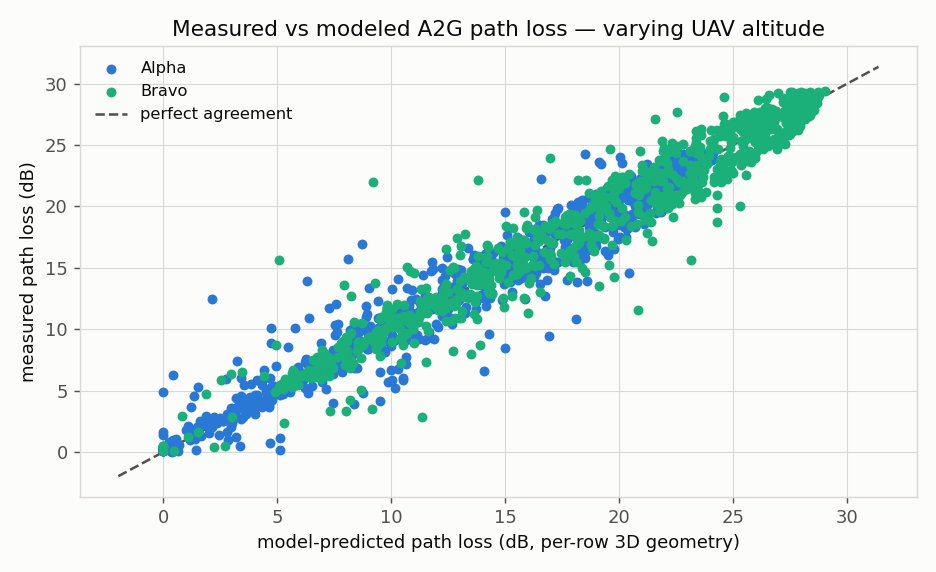
\includegraphics[width=0.86\columnwidth]{parity.png}
\caption{Measured injected path loss vs.\ per-sample model prediction (nomadic run, 1{,}750 samples, three altitudes). On the diagonal; MAE 1.1--1.2~dB.}
\label{fig:parity}
\end{figure}

\begin{figure}[t]
\centering
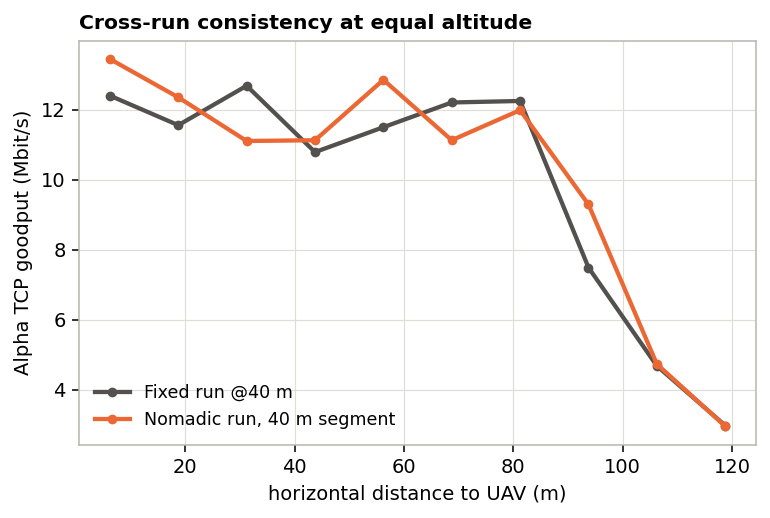
\includegraphics[width=0.78\columnwidth]{consistency.png}
\caption{Cross-run consistency: Alpha's throughput--distance curve from the fixed run and from the nomadic run's 40~m segment coincide.}
\label{fig:consistency}
\end{figure}

\subsection{Fixed versus nomadic operation}
With the UAV fixed at 40~m (Fig.~\ref{fig:fixmov}a), Alpha's throughput holds near the ${\approx}12$~Mbit/s ceiling to ${\sim}85$~m, then collapses over ${\sim}30$~m---a cliff, not a roll-off. When the UAV changes altitude (Fig.~\ref{fig:fixmov}b), the whole cliff \emph{translates}: its knee moves from ${\sim}65$~m (20~m) to ${\sim}95$~m (40~m) to ${\sim}125$~m (60~m). \textbf{Meaning:} a nomadic node does not primarily raise peak rate---it relocates the \emph{boundary} of the usable region. Coverage is a region the operator moves, not a level the operator sets.

\begin{figure}[t]
\centering
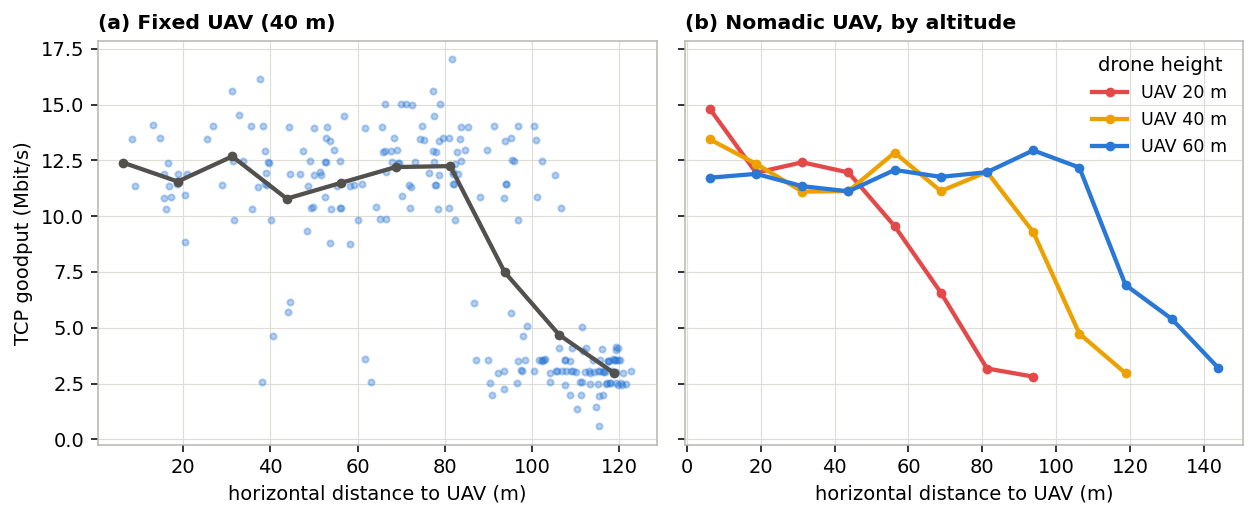
\includegraphics[width=\columnwidth]{fixed_vs_moving.png}
\caption{(a) UAV fixed at 40~m: one cliff near 85~m. (b) UAV free: the cliff moves outward as altitude rises. Higher flight buys range.}
\label{fig:fixmov}
\end{figure}

\subsection{Altitude as a fleet-wide coverage control}
Fig.~\ref{fig:alttput} puts each altitude on its own axis; Fig.~\ref{fig:altploss} shows the underlying path loss; Table~\ref{tab:altitude} isolates the effect at fixed distance. Close to the node altitude is nearly irrelevant; at mid-range (60--90~m) climbing 20$\rightarrow$60~m removes 12~dB and nearly triples throughput ($4.4\rightarrow11.8$~Mbit/s); at far range (90--120~m) it raises throughput almost fivefold ($2.4\rightarrow11.6$) and lifts RSRP by 8~dBm. The mechanism is (3)--(6): a steeper angle drives $P_{\mathrm{LoS}}$ up and strips NLoS excess, which is why the model curve in Fig.~\ref{fig:altploss} is markedly flatter at 60~m than at 20~m. \textbf{Meaning:} for a spread-out fleet, altitude is the lever to reach for first---a robot far across the map but beneath a high UAV is, to the radio, not far at all, and because climbing raises the elevation angle to \emph{every} robot at once it improves the whole fleet's links simultaneously, whereas moving the drone horizontally toward one robot moves it away from another. Our controlled altitude sweep measures this gain directly; a head-to-head lateral-tracking trial is complementary future work. The safe radius grows from 101~m to 163~m across the altitude range.

\begin{figure}[t]
\centering
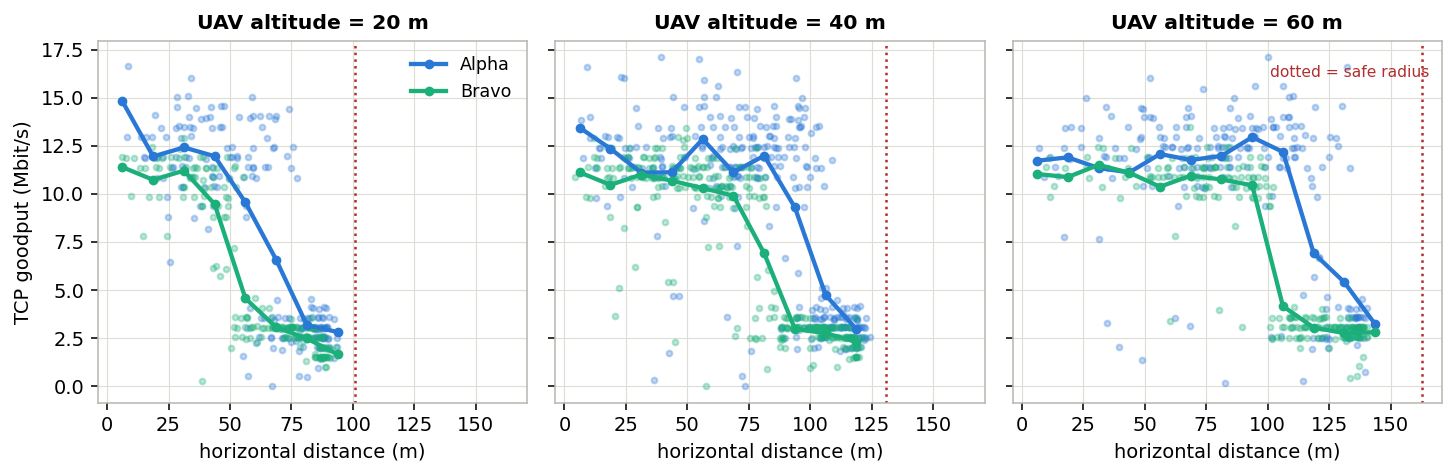
\includegraphics[width=\columnwidth]{per_altitude_tput.png}
\caption{Throughput vs.\ distance, each UAV altitude on its own axis. The coverage knee advances with altitude; Bravo (green) sits below Alpha (blue); dotted line = model safe radius, Eq.~\eqref{eq:rsafe}.}
\label{fig:alttput}
\end{figure}

\begin{figure}[t]
\centering
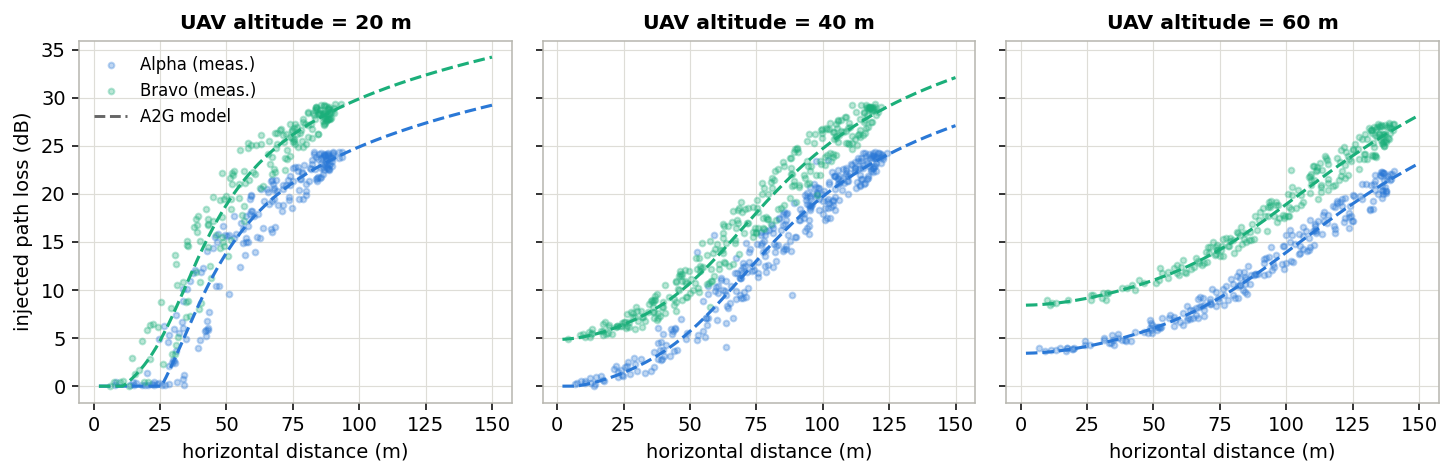
\includegraphics[width=\columnwidth]{per_altitude_ploss.png}
\caption{Measured path loss vs.\ distance per altitude with the analytic model (dashed). Steeper at 20~m (shallow angles, more excess), flatter at 60~m (near-LoS)---the physical basis of the altitude lever.}
\label{fig:altploss}
\end{figure}

\begin{table}[t]
\caption{Altitude effect at equal horizontal distance (Alpha; path loss / TCP / measured RSRP)}
\label{tab:altitude}
\centering
\footnotesize
\begin{tabular}{|l|c|c|c|}
\hline
\textbf{Distance} & \textbf{UAV 20 m} & \textbf{UAV 40 m} & \textbf{UAV 60 m} \\
\hline
20--50 m & 6.2 / 12.1 / $-44$ & 3.4 / 11.4 / $-42$ & 5.2 / 11.4 / $-42$ \\
\hline
60--90 m & \textbf{21.5 / 4.4 / $-58$} & 12.9 / 11.3 / $-50$ & \textbf{9.4 / 11.8 / $-46$} \\
\hline
90--120 m & 24.1 / 2.4 / $-60$ & 20.9 / 5.6 / $-57$ & \textbf{15.2 / 11.6 / $-52$} \\
\hline
\end{tabular}
\end{table}

\subsection{Device budget, coverage, and outages}
The two UEs differ only by 5~dB of baseline budget, yet experience qualitatively different networks (Table~\ref{tab:metrics}). Alpha is distance-limited (goodput $\approx12\rightarrow6$~Mbit/s with range); Bravo is budget-limited (capped lower, reaching the cliff sooner). Over identical trajectories, Bravo suffered 27 outages to Alpha's one. Fairness stays high ($J=0.97$). \textbf{Meaning:} a few dB of device difference relocates the coverage boundary and multiplies the outage rate eightfold; the weakest radio defines the team's safe radius, and high fairness confirms the disparity is device budget, not scheduler bias---so the remedy is coverage margin, not QoS tuning.

\begin{table}[t]
\caption{Measured performance, both runs, both UEs}
\label{tab:metrics}
\centering
\footnotesize
\begin{tabular}{|l|c|c|c|c|}
\hline
\textbf{Metric} & \textbf{Fix$\cdot$A} & \textbf{Fix$\cdot$B} & \textbf{Nom$\cdot$A} & \textbf{Nom$\cdot$B} \\
\hline
TCP goodput mean (Mbit/s) & 8.6 & 6.4 & 8.7 & 6.4 \\
\hline
Video $\ge$7.9 Mbit/s & 100\% & 100\% & 100\% & 100\% \\
\hline
Uplink RTT mean/p95 (ms) & 31/46 & 32/46 & 32/47 & 34/47 \\
\hline
C2 RTT med/p95 (ms) & 39/52 & 37/49 & 39/52 & 37/50 \\
\hline
PDR UL/DL (\%) & 99.6/97.9 & 99.6/98.8 & 99.8/98.3 & 96.5/95.7 \\
\hline
RSRP range (dBm) & $-42/-61$ & $-42/-66$ & $-42/-61$ & $-42/-66$ \\
\hline
SINR mean (dB) & 39 & 34 & 39 & 35 \\
\hline
Outage prob. & 0.0\% & 0.4\% & 0.1\% & 3.1\% \\
\hline
Conn.\ reliability & 100\% & 99.6\% & 99.9\% & 96.9\% \\
\hline
\end{tabular}
\end{table}

\subsection{Traffic-class behaviour and early warning}
The three traffic classes fail in distinct, ordered ways. Video is all-or-nothing: full 8~Mbit/s inside the envelope, absent at the edge. TCP bends gracefully ($\approx12\rightarrow5\rightarrow1$~Mbit/s). C2 command delivery is most robust---median 37--39~ms, p95 $\le52$~ms, indifferent to distance and altitude---until immediately before the edge, where its RTT inflates by an order of magnitude (to several hundred ms) \emph{before} any packet is lost. \textbf{Meaning:} edge approach is legible as a fixed sequence---video drops, transfers crawl, commands lag. Because C2 (the steer/stop channel) degrades in \emph{latency} before it loses \emph{packets}, the network provides an intrinsic early-warning signal for loss of controllability, on which a predictive controller can act before command delivery actually fails.

\section{Discussion}
These results refine the mental model of an aerial base station as ``coverage that follows you.'' Because the radio responds to elevation angle rather than map distance, altitude is a distinctively fleet-wide lever: climbing raises the angle---and lowers excess loss---to every robot simultaneously, whereas repositioning the node horizontally improves one user's geometry at the expense of another's. Two operating rules follow. First, for a distributed fleet, climbing is the first response when users struggle---a geometric argument our altitude sweep supports directly and that a controlled lateral-tracking trial would test head-to-head. Second, because failure at the boundary is abrupt but pre-announced, control should be predictive: the C2-latency and HARQ-rate leading indicators, the altitude lever, and the hard safe-radius constraint~\eqref{eq:rsafe} are exactly the ingredients for a learning-based nomadic-node controller, for which the labelled corpus collected here is a training substrate. A corollary for repositioning: since coverage moves with the node and descent shrinks it, the safe manoeuvre is climb--translate--descend, descending last when users are closest.

\section{Limitations}
\emph{Open-field LoS only.} Every measurement was taken in an obstacle-free field; the NLoS term of~(6) is present but never dominates. The findings characterize the clean A2G regime and do not yet speak to urban canyons, canopy, rubble, or building shadowing, where multipath and blockage would reshape the edge and could complicate the altitude lever (a higher UAV sees over some obstacles but lengthens the slant path). The quantitative edges are best-case, LoS figures. \emph{Further caveats.} The RAN runs over \texttt{rfsimulator}, so fast fading beyond configured profiles is absent and numeric edges are specific to this configuration and calibration; the UAV holds altitude statically; robot speed (1~m/s) exceeds the TurtleBot3 specification; SINR reproduces the device gap but its absolute scale is compressed by power control and is not treated as calibrated; RSRQ, F1/midhaul (no CU/DU split), UAV energy, NR-U coexistence, and a simulation-to-hardware gap are out of scope; the 1.2~dB figure is internal consistency, not sim-to-hardware. Subject to the LoS scope, none of these affects the \emph{direction} of the findings, which follow from geometry, link budget, and protocol-state mechanisms that carry to physical LoS deployments.

\section{Conclusion and Future Work}
\label{sec:conclusion}
We presented, in full methodological detail, a mobility-coupled 5G emulation testbed for UAV-mounted base stations serving ground robots, and over a 7.5-hour open-field LoS campaign---validated to 1.2~dB and corroborated by the modem's RSRP---established that UAV altitude is a powerful, fleet-wide coverage control: climbing recovers margin, triples mid-range throughput, and moves the coverage cliff and safe radius outward while improving every robot's link at once---in contrast to horizontal repositioning, which trades quality between users (a controlled head-to-head of the two is complementary future work). We further showed a small device-budget gap multiplies the outage rate, that traffic classes fail in an ordered sequence that provides early warning of lost controllability, and that node repositioning must be coordinated; and we documented three silent-failure pitfalls of single-host RAN emulation with remedies. The central next step is to relax the line-of-sight assumption with realistic clutter and an NLoS-dominant channel, determining how much of the clean-field coverage rule survives---alongside a coverage-edge recovery-time study, a CU/DU split for midhaul metrics, and eventual SDR hardware validation.

\section*{Acknowledgment}
Supported by the Telkom--NRF FutureTech Programme and DIGITAfrica (Horizon Europe). The authors thank the OpenAirInterface and Open5GS communities.

\begin{thebibliography}{00}
\bibitem{zeng2016wireless} Y. Zeng, R. Zhang, and T. J. Lim, ``Wireless communications with unmanned aerial vehicles: Opportunities and challenges,'' \textit{IEEE Commun. Mag.}, vol.~54, no.~5, pp.~36--42, 2016.
\bibitem{zeng2019accessing} Y. Zeng, Q. Wu, and R. Zhang, ``Accessing from the sky: A tutorial on UAV communications for 5G and beyond,'' \textit{Proc. IEEE}, vol.~107, no.~12, pp.~2327--2375, 2019.
\bibitem{mozaffari2019tutorial} M. Mozaffari, W. Saad, M. Bennis, Y.-H. Nam, and M. Debbah, ``A tutorial on UAVs for wireless networks: Applications, challenges, and open problems,'' \textit{IEEE Commun. Surveys Tuts.}, vol.~21, no.~3, pp.~2334--2360, 2019.
\bibitem{alhourani2014optimal} A. Al-Hourani, S. Kandeepan, and S. Lardner, ``Optimal LAP altitude for maximum coverage,'' \textit{IEEE Wireless Commun. Lett.}, vol.~3, no.~6, pp.~569--572, 2014.
\bibitem{3gpp36777} 3GPP, ``Study on enhanced LTE support for aerial vehicles,'' TR~36.777, 2017.
\bibitem{nikaein2014oai} N. Nikaein \textit{et al.}, ``OpenAirInterface: A flexible platform for 5G research,'' \textit{ACM SIGCOMM Comput. Commun. Rev.}, vol.~44, no.~5, pp.~33--38, 2014.
\bibitem{open5gs} Open5GS, ``Open source implementation of the 5G core network,'' \url{https://open5gs.org}, accessed 2026.
\bibitem{koenig2004gazebo} N. Koenig and A. Howard, ``Design and use paradigms for Gazebo, an open-source multi-robot simulator,'' in \textit{Proc. IEEE/RSJ IROS}, 2004, pp.~2149--2154.
\end{thebibliography}

\end{document}
